\documentclass{bmstu}


\usepackage{physics}
\usepackage{pdfpages}
\usepackage{tabularx}
\usepackage{longtable}
\usepackage{xfrac}
\usepackage{amssymb}
\usepackage{dsfont}
\usepackage{upgreek}
\usepackage{color, colortbl}
\usepackage{graphicx}
\usepackage{listings}
\usepackage{ amssymb }
\usepackage{tikz}

\graphicspath{
	{graphics/}
}

\begin{document}
	
	\section*{25/10}
	Связь между координатами:
	\[
	\begin{cases}
		L_i+L_j+L_k=1 \\
		x=L_ix_i+L_jx_j+L_kx_k \\
		y=L_iy_i+L_jy_j+L_ky_k
	\end{cases}
	\]
	
	$V=hdS, h=\text{const}-\text{толщина элемента}$
	
	\[
	h\iint\limits_Sf(x,y)\ dxdy= h\int\limits_0^1\int\limits_0^{1-L_j} f(L_i,L_j,L_k)|J|\ dL_iL_j
	\]
	\[
	J=\begin{bmatrix}
		\dfrac{\partial x}{\partial L_i} & \dfrac{\partial x}{\partial L_j} \\
		
		\dfrac{\partial y}{\partial L_i} & \dfrac{\partial y}{\partial L_j}
	\end{bmatrix} = \begin{bmatrix}
	x_i-x_k & x_j-x_k \\
	y_i-y_k & y_j-y_k
	\end{bmatrix} \Rightarrow |J|=\Delta
	\]
	
\begin{minipage}{0.45\textwidth}
    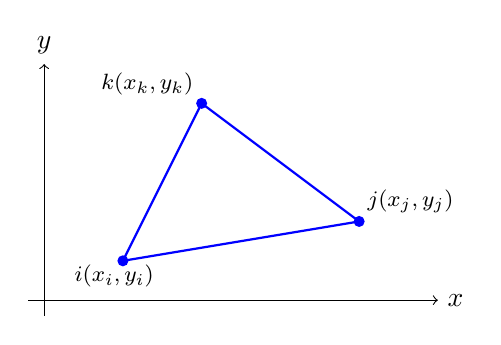
\begin{tikzpicture} 
        \draw[->] (-0.2,0) -- (5,0) node[right] {$x$};
        \draw[->] (0,-0.2) -- (0,3) node[above] {$y$};
        \draw[blue, thick] (1,0.5) -- (4,1) -- (2,2.5) -- cycle;
        {\footnotesize
        \node at (1.5,0.55) [below left] {$i(x_i, y_i)$};
        \node at (4,1) [above right] {$j(x_j, y_j)$};
        \node at (2,2.5) [above left] {$k(x_k, y_k)$};
        }
        \fill[blue] (1, 0.5) circle (2pt);
        \fill[blue] (4,1) circle (2pt);
        \fill[blue] (2,2.5) circle (2pt);
    \end{tikzpicture}
\end{minipage}
\hfill
\begin{minipage}{0.45\textwidth}
    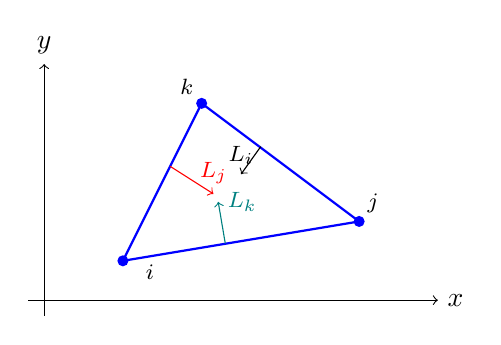
\begin{tikzpicture}
        \draw[->] (-0.2,0) -- (5,0) node[right] {$x$};
        \draw[->] (0,-0.2) -- (0,3) node[above] {$y$};
        \draw[blue, thick] (1,0.5) -- (4,1) -- (2,2.5) -- cycle;
        {\footnotesize
        \node at (1.5,0.55) [below left] {$i$};
        \node at (4,1) [above right] {$j$};
        \node at (2,2.5) [above left] {$k$};
        }
        \fill[blue] (1, 0.5) circle (2pt);
        \fill[blue] (4,1) circle (2pt);
        \fill[blue] (2,2.5) circle (2pt);

        \draw[->, thin, teal] (2.3, 0.72) -- (2.21,1.25) node[right] {\footnotesize $L_k$};
        \draw[->, thin, red] (1.6, 1.7) -- (2.15,1.35) node[above] {\footnotesize $L_j$};
        \draw[->, thin] (2.75, 1.95) -- (2.5,1.6) node[above] {\footnotesize $L_i$};
    \end{tikzpicture}
\end{minipage}

\begin{center}
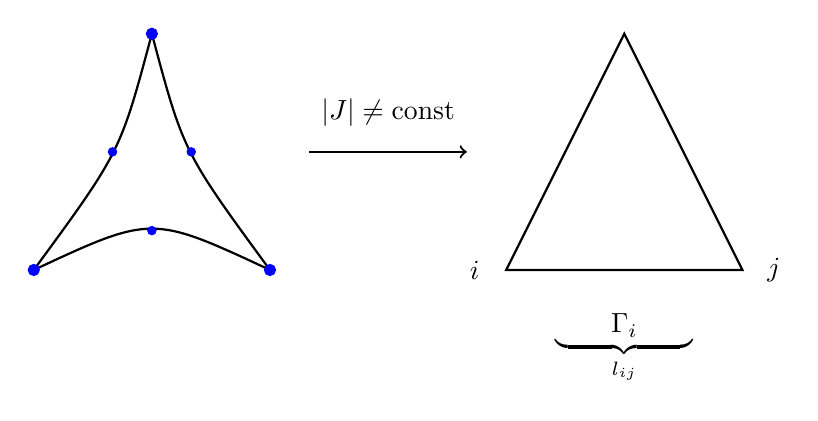
\begin{tikzpicture}
    % Вогнутый треугольник
    \draw[thick] (0,0) .. controls (1.5,0.7) and (1.5,0.7) .. (3,0)   % нижняя вогнутая сторона
                 .. controls (1.9,1.5) and (1.9,1.5) .. (1.5,3)         % правая вогнутая сторона
                 .. controls (1.1,1.5) and (1.1,1.5) .. (0,0);        % левая вогнутая сторона

    % Точки на вершинах
    \filldraw[blue] (0,0) circle (2pt);   % Нижняя левая вершина
    \filldraw[blue] (3,0) circle (2pt);   % Нижняя правая вершина
    \filldraw[blue] (1.5,3) circle (2pt); % Верхняя вершина

    % Промежуточные точки
    \filldraw[blue] (1.5,0.5) circle (1.5pt);   % Точка на нижней стороне
    \filldraw[blue] (2,1.5) circle (1.5pt);   % Точка на правой стороне
    \filldraw[blue] (1.,1.5) circle (1.5pt);   % Точка на левой стороне
    
    \draw[->][thick] (3.5, 1.5) -- (5.5, 1.5);
    \node at (4.5, 2) {$|J| \neq \text{const}$}; 
    \node at (5.6, 0) {$i$}; 
    \node at (9.4, 0) {$j$}; 
    \node at (7.5, -1) {$\underbrace{\qquad \Gamma_i \qquad}_{l_{ij}}$}; 
    
     \draw[thick] (6,0) -- (7.5,3) -- (9,0) -- cycle;
\end{tikzpicture}
\end{center}
	
	
	Интегральные формулы, упрощающие вычисления:
	\[
	\int\limits_{\Gamma_{ij}} L_i^{\alpha}L_j^{\beta} \ d\Gamma = \frac{\alpha!\beta!}{(\alpha+\beta+1)!}\cdot l_{ij}
	\]
	\[
		\int\limits_{S} L_i^{\alpha}L_j^{\beta}L_k^{\gamma} \ dS = \frac{\alpha!\beta!\gamma!}{(\alpha+\beta+\gamma+2)!}\cdot 2S \tag{1}
	\]
	
	
	Возвращаемся к формуле из прошлой лекции:
	\[
	\int\limits_{\Omega}  N^T N\ dx dy = \int\limits_{\Omega}  
	\begin{bmatrix}
		N_iN_i & N_iN_j & N_iN_k \\
		N_iN_j & N_jN_j & N_jN_k \\
		N_iN_k & N_jN_k & N_kN_k \\
	\end{bmatrix}
	\ dx dy = 
	\]
	\[
	= \int\limits_S \begin{bmatrix}
		L_iL_i & L_iL_j & L_iL_k \\
		L_iL_j & L_jL_j & L_jL_k \\
		L_iL_k & L_jL_k & L_kL_k \\
	\end{bmatrix} |J| \ dL_i L_j = \dfrac{S}{12} \begin{bmatrix}
	2 & 1 & 1 \\ 1 & 2 & 1 \\ 1 & 1 & 2
	\end{bmatrix}
	\]
	
	Вычисляем компоненты матрицы по формуле (1):
	\[
	\int\limits_{\Omega} L_i^2 \ dS = \int\limits_{\Omega} L_i^2L_j^0L_k^0 \ dS=  \dfrac{2!\, 0!\, 0!}{(2+0+0+2)!}\cdot 2S=\frac{S}{6}
	\]
	\[
	\int\limits_SN^{\text{T}} \ dS = \int\limits_S \begin{bmatrix}
		N_i \\ N_j \\ N_k
	\end{bmatrix} \, dxdy = \int\limits_S \begin{bmatrix}
	L_i \\ L_j \\ L_k
	\end{bmatrix} \, dS = \frac{S}{3} \begin{bmatrix}
	1 \\ 1 \\ 1
	\end{bmatrix}
	\]
	
	\[
	\int\limits_{\Gamma} \left(K_x \cdot  \frac{\partial u}{\partial x} \cdot l_x + K_y \cdot  \frac{\partial u}{\partial y} \cdot l_y \right)v\ d\Gamma 
	\]
	\begin{enumerate}
		\item или $K_x \cdot  \frac{\partial u}{\partial x} \cdot l_x + K_y \cdot  \frac{\partial u}{\partial y} \cdot l_y=\hat\sigma$ или $q$ 
		\item или $K_x \cdot  \frac{\partial u}{\partial x} \cdot l_x + K_y \cdot  \frac{\partial u}{\partial y} \cdot l_y=-\alpha_g(u-\hat u)$ 
	\end{enumerate}
	
	Рассмотрим подробнее:
	\begin{enumerate}
		\item $
		\displaystyle\int\limits_{\Gamma} \hat \sigma \ d\Gamma = \{\delta \Phi\}^T \int\limits_{\Gamma} \hat \sigma N^T\ d\Gamma\int\limits_{\Gamma} \begin{bmatrix}
			L_i \\ L_j \\ L_k
		\end{bmatrix} \, d\Gamma$
		\begin{enumerate}
			\item $\displaystyle\int\limits_{\Gamma_{ij}} \begin{bmatrix}
				L_i \\ L_j \\ 0
			\end{bmatrix} \, d\Gamma = 
			\begin{vmatrix}
			\displaystyle\int\limits_{\Gamma_{ij}} L_i^1 L_j^0 d\Gamma = \frac{1!}{(1+1)!} l_{ij}
			\end{vmatrix}= \dfrac{l_{ij}}{2}\begin{bmatrix}
			1\\1\\0
		\end{bmatrix}$
		\item $\displaystyle\int\limits_{\Gamma_{jk}} \begin{bmatrix}
				0 \\ L_j \\ L_k
			\end{bmatrix} \, d\Gamma = \dfrac{l_{jk}}{2}\begin{bmatrix}
			0\\1\\1
		\end{bmatrix}$
		\item $\displaystyle\int\limits_{\Gamma_{ik}} \begin{bmatrix}
				L_i \\ 0 \\ L_k
			\end{bmatrix} \, d\Gamma = \dfrac{l_{jk}}{2}\begin{bmatrix}
			1\\0\\1
		\end{bmatrix}$
		\end{enumerate}
	\[\int \limits_{\Gamma} \alpha_g (u - \hat u) v d \Gamma = \int \limits_{\Gamma} \alpha_g u \cdot v d \Gamma - \int \limits_{\Gamma} \alpha_g \hat u \cdot v d \Gamma = \]
	\[=\delta\Phi^T \left(\int \limits_{\Gamma} \alpha_g N^T N d\Gamma \cdot \Phi - \alpha_g \hat u \int \limits_{\Gamma} N^T d\Gamma \right)\]
	\[\int \limits_{\Gamma} \alpha_g N^T N d\Gamma = \int \limits_{\Gamma} \begin{bmatrix}
	L_iL_i & L_iL_j & L_iL_k\\
	0 & L_j^2 & L_jL_k\\
	0 & 0 & L_k^2
	\end{bmatrix}
	d\Gamma
	\]
	\begin{enumerate}
	\item \[\int \limits_{\Gamma_{ij}} \begin{bmatrix}
	L_iL_i & L_iL_j & 0\\
	0 & L_j^2 & 0\\
	0 & 0 & 0
	\end{bmatrix}
	d\Gamma = 
	\begin{vmatrix} \displaystyle
			\ \int\limits_{\Gamma_{ij}} L_i^2L_j^0 d\Gamma = \frac{2!\cdot 0!}{(2+1)!} l_{ij} = \frac{2}{6}l_{ij}\\
			\ \displaystyle \int\limits_{\Gamma_{ij}} L_i^1L_j^1 d\Gamma = \frac{1! \cdot 1!}{(1+1+1)!} l_{ij} = \frac{1}{6}l_{ij}
			\end{vmatrix}=\]
	\[= \frac{2}{6}l_{ij} 
	\begin{bmatrix}
	2 & 1 & 0\\
	1 & 2 & 0\\
	0 & 0 & 0
	\end{bmatrix}
	\]
	(b), (c) -- аналогично
	\end{enumerate}
	\end{enumerate}
	
	
	
\end{document}